\documentclass[11pt]{article}
\usepackage[a4paper, margin=0.5in]{geometry}
\usepackage{cite}
\usepackage{amsmath,amssymb,amsfonts}
\usepackage{algorithmic}
\usepackage[export]{adjustbox}
\usepackage{graphicx}
\usepackage{textcomp}
\usepackage{listings}
\usepackage{matlab-prettifier}
\usepackage{tabularx}
\usepackage{caption}
\usepackage{subcaption}
\usepackage{url}
\usepackage{hyperref}
\usepackage{array}
\usepackage{lastpage}
\raggedbottom
\usepackage{cite}
\usepackage{indentfirst}
\usepackage{fancyhdr}
\renewcommand*\contentsname{TABLE OF CONTENTS}
\renewcommand{\listfigurename}{List of Figures}
\begin{document}
\tableofcontents
\listoffigures
\pagestyle{fancy}
\fancyhead{}
\fancyhead[LO,LE]{Name: Md. Raisul Islam Rifat}
\fancyhead[RO,RE]{ID: 1902081}
\fancyfoot{}
\fancyfoot[RE,RO]{Page \thepage\ of \pageref{LastPage}}
\newpage
\setcounter{page}{1}
\section{Abstract}
This document presents the layout design of a 2-input NAND gate in Cadence Virtuoso, utilizing the 90nm architecture. Building upon the results of a prior experiment, which involved the schematic design of the NAND gate using NMOS and PMOS transistors, this research aims to translate the schematic design into an optimized layout. Leveraging the advanced features of the 90nm technology node, the layout was meticulously crafted to optimize area, power consumption, and propagation delay while ensuring robustness against process variations. Rigorous simulations were conducted to validate the functionality and performance of the layout, demonstrating its efficacy in modern integrated circuit design.
\section{Keywords}
2-input NAND gate, Layout design, Cadence Virtuoso, 90nm architecture, Integrated circuit design, NMOS and PMOS transistors.
\section{Objectives}
\begin{enumerate}
    \item To create a layout view of the basic two input NAND circuit from scratch.
    \item To perform the design rule check (DRC) of the NAND gate layout.
    \item To perform the layout vs. schematic (LVS) check for the NAND gate layout.
    \item To perform parasitic extraction on the NAND gate layout.
\end{enumerate}
\section{Introduction}
By performing this experiment, we will learn about the usage of
CADENCE VIRTUOSO. We will also learn about layout design process. We will also learn about the design rule check (DRC), layout vs. schematic (LVS) check and parasitic extraction. We will also observe the extracted layout design.
\section{Theory}
NAND gate is a fundamental digital logic gate used extensively in digital
circuits due to its versatility and functional completeness. A NAND gate
performs the logical NAND operation, where the output is true (or high)
unless both inputs are true (or high). This gate is a building block for
various digital systems, including arithmetic logic units, memory storage,
and more complex logic circuits. Designing a 2-input NAND gate in Cadence Virtuoso, an advanced electronic design automation (EDA) tool,
involves a series of methodical steps, from schematic capture to simulation.
Cadence Virtuoso offers a comprehensive environment for the design and
verification of custom ICs, providing tools for schematic entry, layout
editing, and extensive simulation capabilities. The process begins with
creating a transistor-level schematic of the NAND gate using PMOS and
NMOS transistors. This is followed by generating a symbol for the NAND
gate, enabling its use in hierarchical design contexts. The next step is the
simulation. This step is followed by the layout design process. This process contains the actual designing process as well as different types of checking and verification process.
\newpage
\section{Truth Table}
\begin{center}
    \begin{tabular}{|c|c|c|c|c|}
        \hline
        \hline
        A (input) & B (input) & Pull Down Network & Pull Up Network & O (output) \\
        \hline
        \hline
        0         & 0         & Off               & On              & 1          \\
        \hline
        0         & 1         & Off               & On              & 1          \\
        \hline
        1         & 0         & Off               & On              & 1          \\
        \hline
        1         & 1         & On                & Off             & 0          \\
        \hline
    \end{tabular}
\end{center}
\section{Layout Design}
\begin{figure}[!h]
    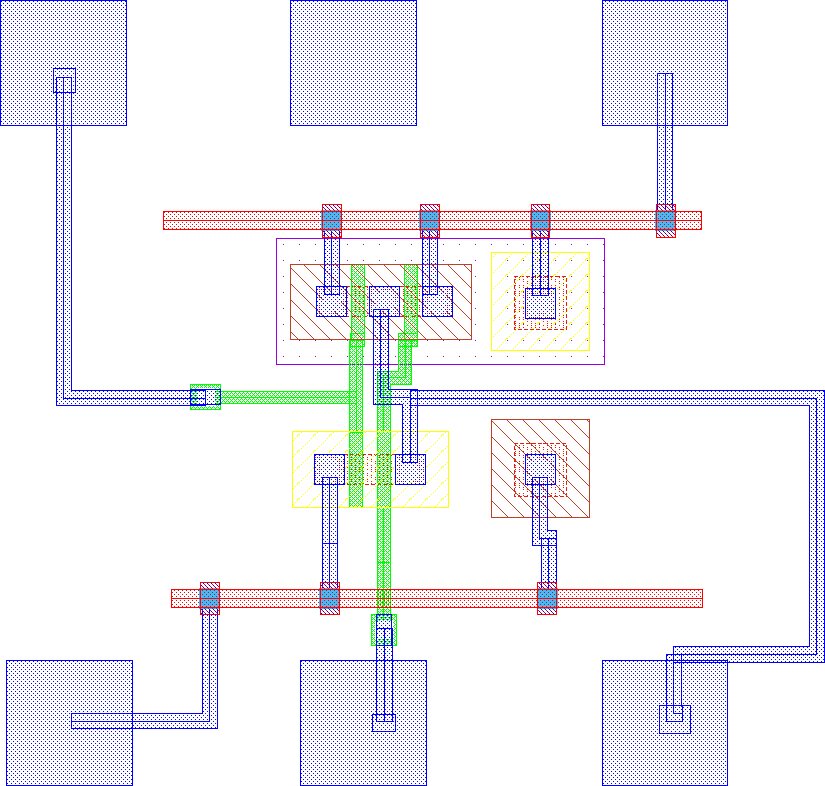
\includegraphics[width=\textwidth,inner]{layout}
    \caption{Layout of 2-input NANAD gate.}
\end{figure}
\newpage
\section{Layout Design Check}
\subsection{Design Requirement Check}
\begin{figure}[!h]
    \begin{subfigure}[h]{\textwidth}
        \begin{center}
            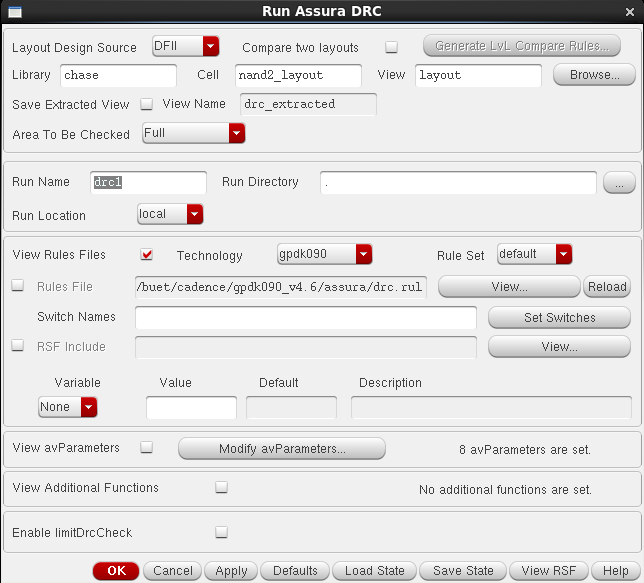
\includegraphics[width=0.5\textwidth]{drc}
            \caption{Assura DRC setup.}
        \end{center}
    \end{subfigure}
    \begin{subfigure}[h]{\textwidth}
        \begin{center}
            \vspace{1in}
            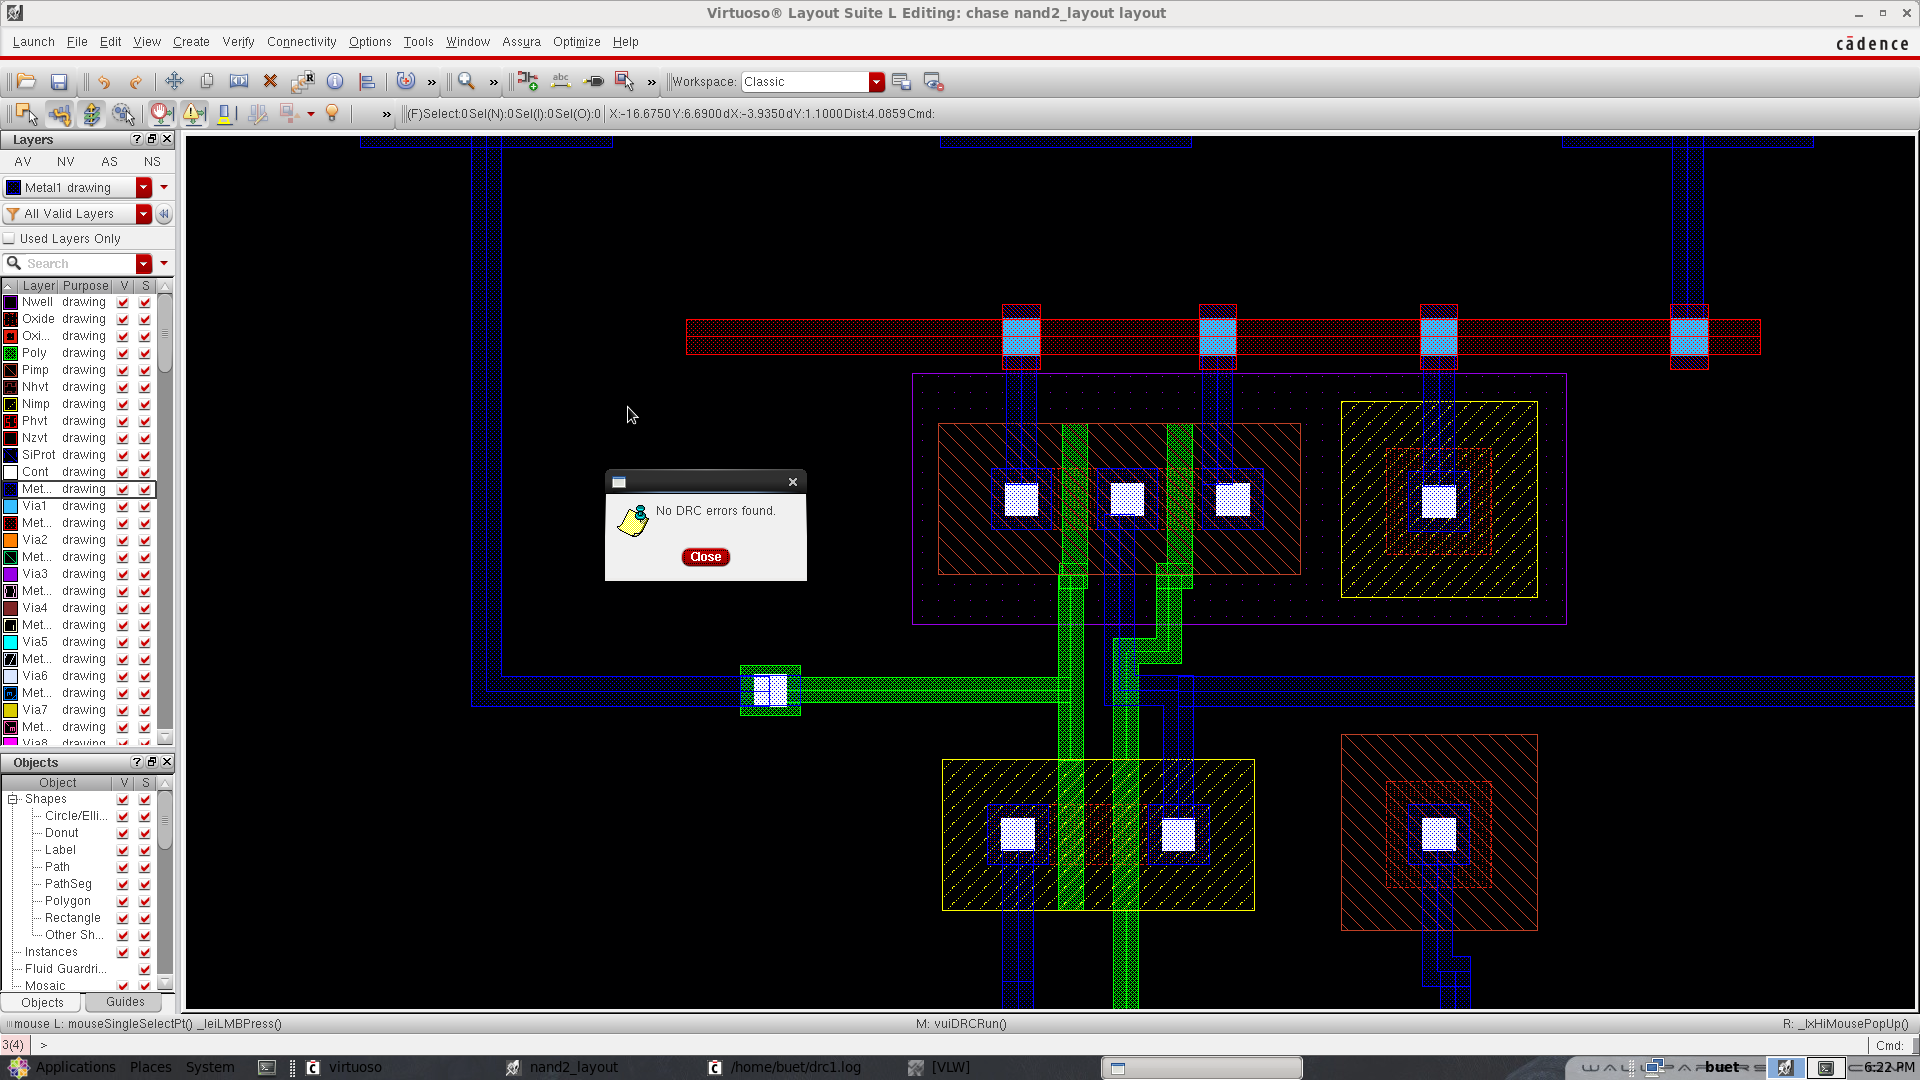
\includegraphics[width=\textwidth]{drcResult}
            \caption{Assura DRC check result.}
        \end{center}
    \end{subfigure}
    \caption{Assura Design Requirement Check (DRC) setup and result.}
\end{figure}
\newpage
\subsection{Layout Vs. Simulation check}
\begin{figure}[!h]
    \begin{subfigure}[h]{\textwidth}
        \begin{center}
            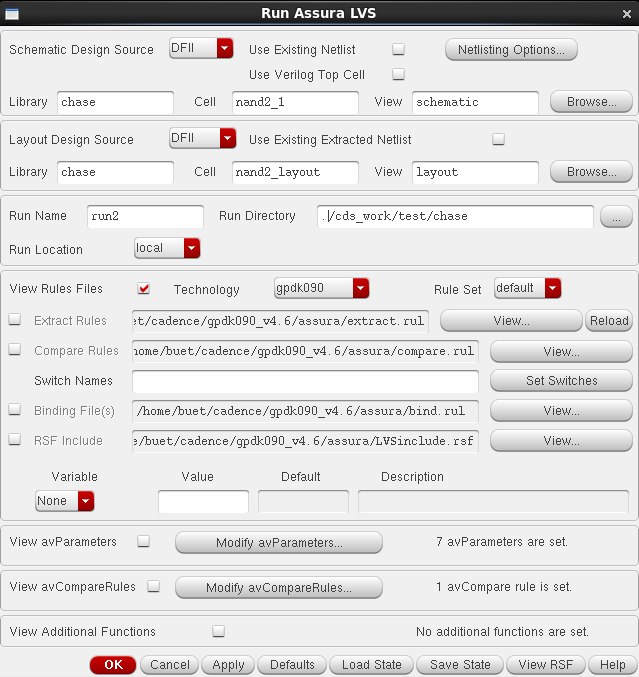
\includegraphics[width=0.5\textwidth]{lvsSetup}
            \caption{Assura LVS setup.}
        \end{center}
    \end{subfigure}
    \begin{subfigure}[h]{\textwidth}
        \begin{center}
            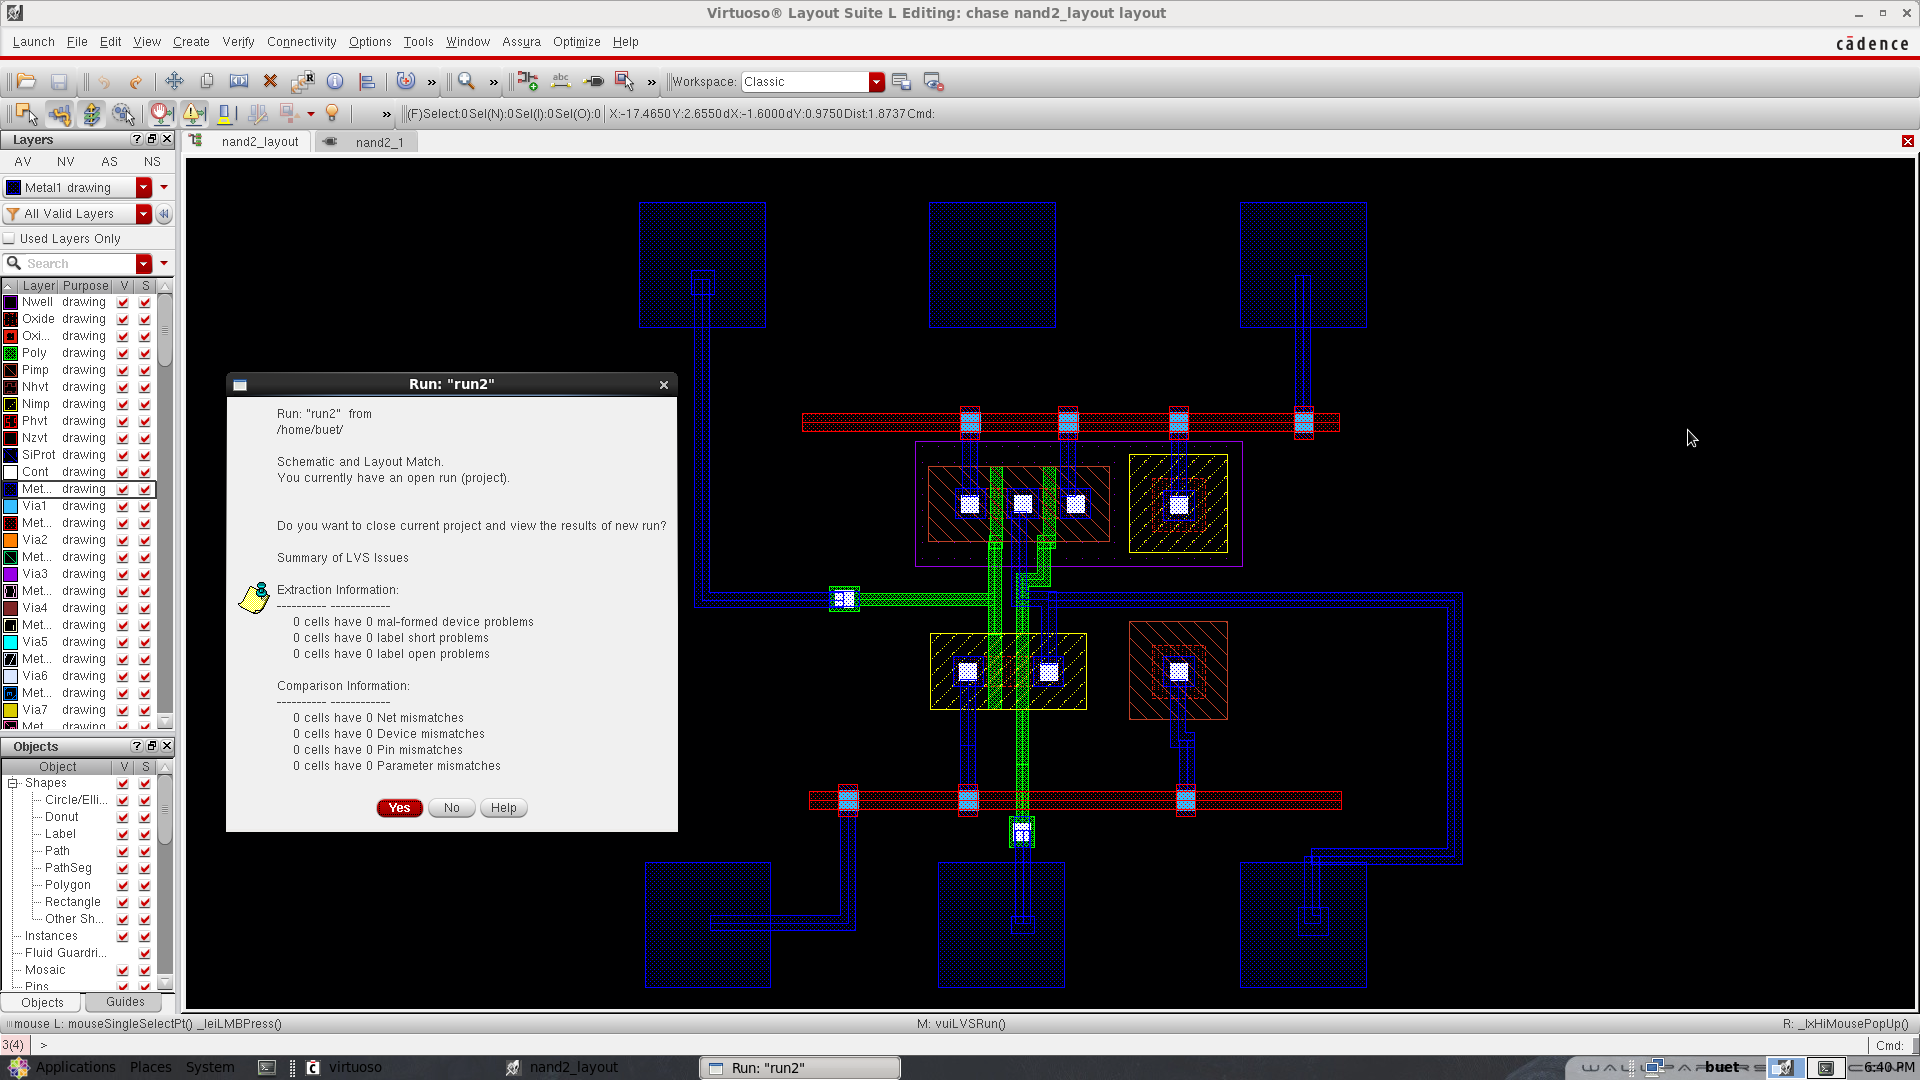
\includegraphics[width=\textwidth]{LVSoutput}
            \caption{Assura LVS check result.}
        \end{center}
    \end{subfigure}
    \caption{Assura Layout Vs. Schematic (LVS) check setup and result.}
\end{figure}
\newpage
\subsection{RCX Run and Parasitic Extraction}
\begin{figure}[!h]
    \begin{subfigure}[h]{\textwidth}
        \begin{center}
            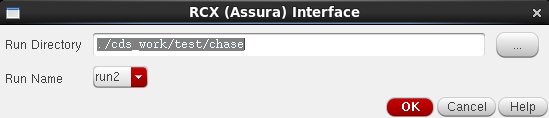
\includegraphics[scale=0.5]{rcxInterface}
            \caption{RCX interface.}
        \end{center}
    \end{subfigure}
    \begin{subfigure}[h]{0.5\textwidth}
        \begin{center}
            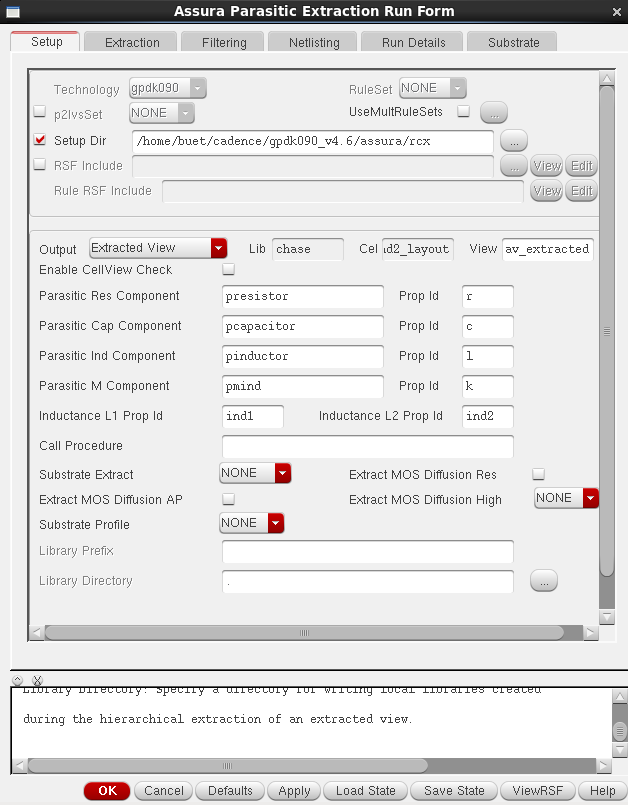
\includegraphics[width=0.95\textwidth,height=4in]{rcxSetup}
            \caption{Assura Parasitic Extraction Run Form -- Setup tab.}
        \end{center}
    \end{subfigure}
    \begin{subfigure}[h]{0.5\textwidth}
        \begin{center}
            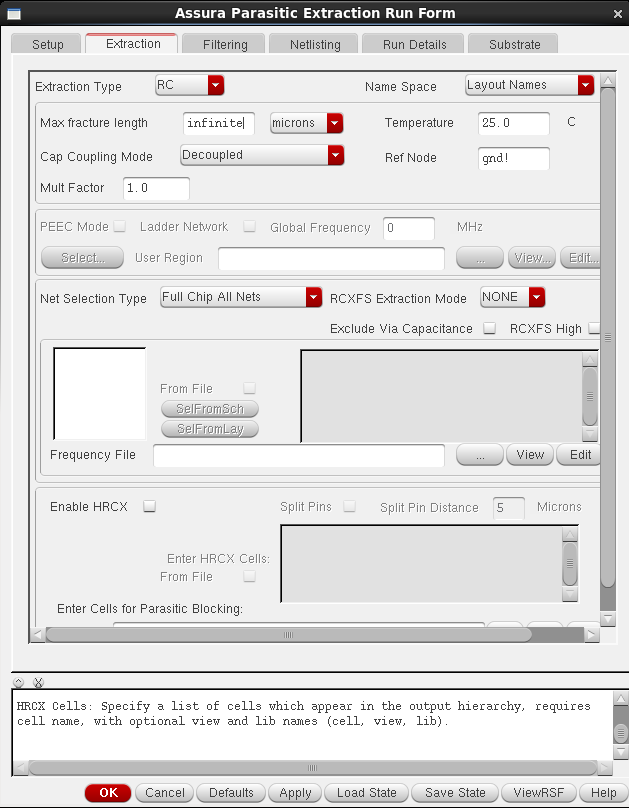
\includegraphics[width=0.95\textwidth,height=4in]{rcxExtraction}
            \caption{Assura Parasitic Extraction Run Form -- Extraction tab.}
        \end{center}
    \end{subfigure}
    \vspace{0.1in}
    \begin{subfigure}[h]{\textwidth}
        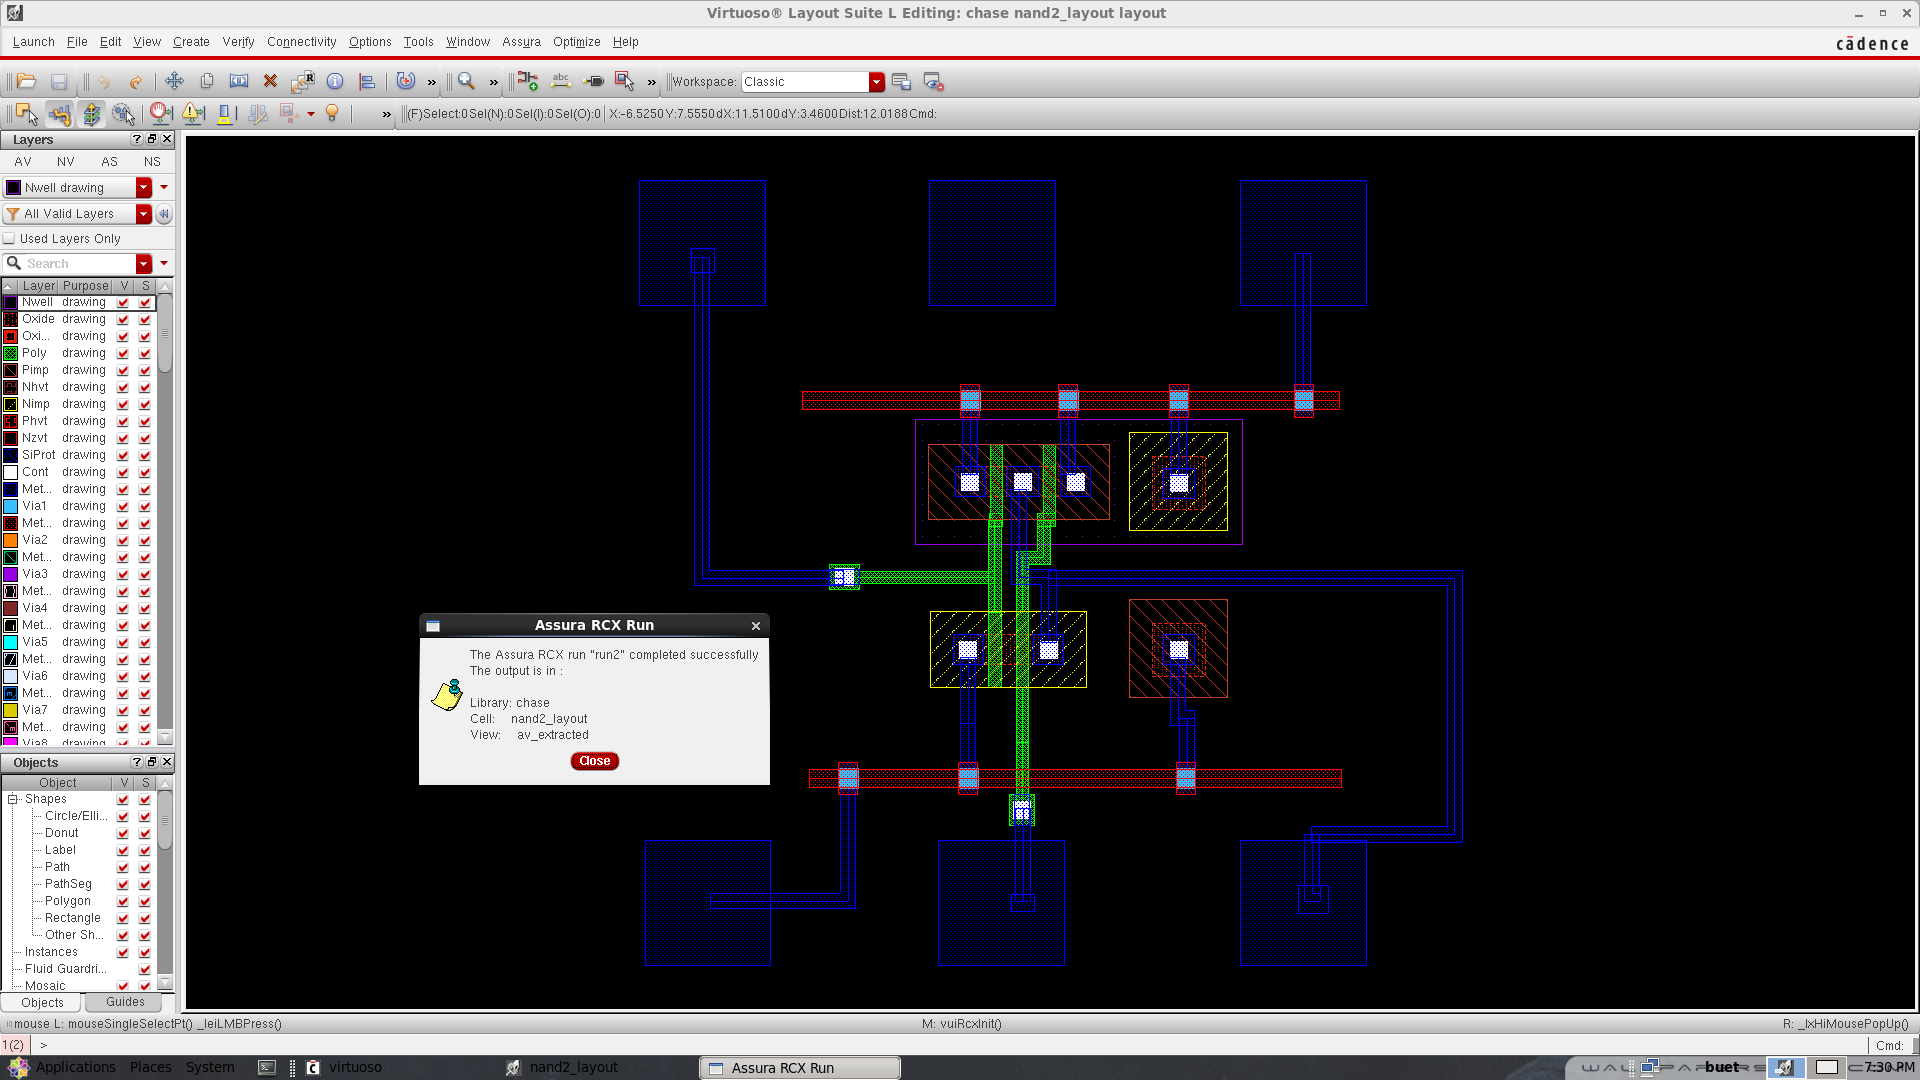
\includegraphics[width=\textwidth]{rcxOutput}
        \caption{Assura RCX Run result.}
    \end{subfigure}
    \caption{Assura RCX and Parasitic Extraction setup and result.}
\end{figure}
\begin{figure}[!h]
    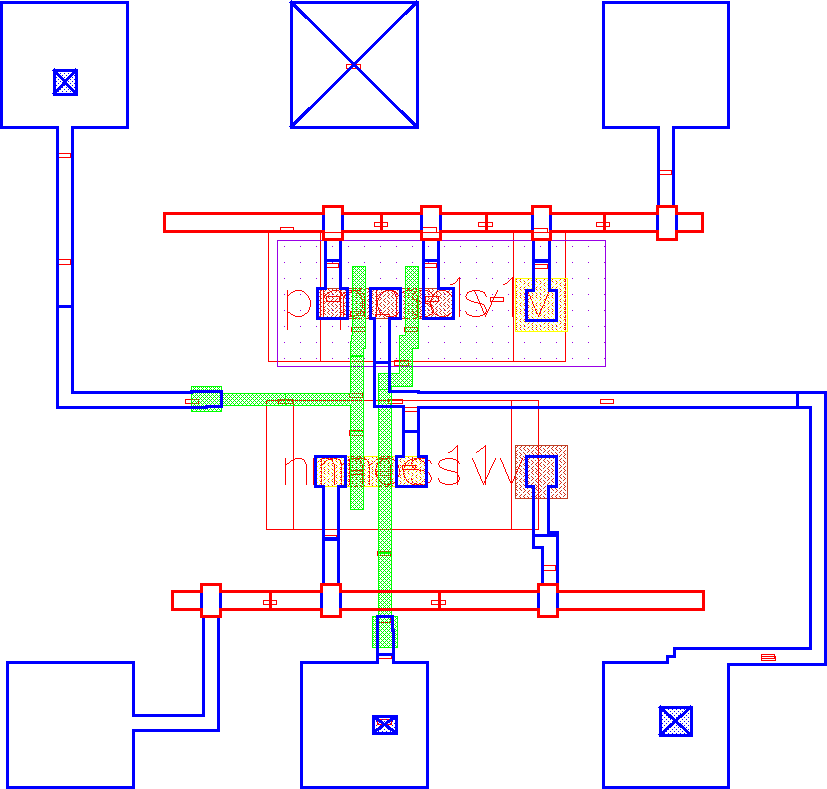
\includegraphics[width=\textwidth]{avExtracted}
    \caption{AV Extracted Layout.}
\end{figure}
\newpage
\section{Conclusion}
In this experiment, we became acquainted with Cadence Software . We
created the layout for a 2-input NAND gate and identified the required designed
parameters and requirements. We also performed DRC, LVS, RCX, and parasitic extraction.
\section{References}
\begin{enumerate}
    \item Lab Manual.
    \item Cadence Virtuoso Tutorial - University of Southern California.
\end{enumerate}
\end{document}